\chapter{Data Handling}

\section{Classification}
Do understand how to protect data several security policies \textbf{classify data} into \textit{four }categories according the need for
\textbf{confidentiality} and the resulting risk profile:
\labelitemize{\textit{Security needs classification}}{
   \begin{enumerate}
      \item \textbf{Public Data}\\
      Data can be disclosed without restriction.
      \note{Directories,
      Maps, Syllabi and Course Materials, de-identified data sets}
      \item \textbf{Internal Data}\\
      Confidentiality of data is preferred, but information contained in
      data may be subject to open records disclosure.
      \note{email
      correspondence, budget plans, employee EmplID}
      \item \textbf{Sensitive Data}\\
      Data confidentiality required by law, policy, or contractual
      obligation
      \item \textbf{Restricted Data}\\
      Restricted data requires privacy and security protections.
      Special authorization may be required for use and collection.
      \note{data
      sets with individual Social Security Numbers (or last four of SSN), credit card
      transaction or cardholder data, patient health data, financial data}
   \end{enumerate}
}

Another classification is the one based on the availability needed for data:
\labelitemize{Availability needs classification}{
   \begin{enumerate}
      \item \textbf{Supportive Data}\\
      Data that is necessary for day-to-day operations, but
      is not critical to the mission or core functions.
      \item \textbf{High-priority Data}\\
      Availability of data is necessary for organization function. 
      Destruction or temporary loss of data may have an adverse
      affect on organization mission, but would not affect organization-wide
      function.
      \item \textbf{Critical Data}\\
      Critical data has the highest need for availability. If the
      information is not available due to system downtime, modification,
      destruction, etc., the organization functions and mission would be
      impacted. Availability of this information must be rigorously protected.
   \end{enumerate}   
}

\section{Protection}
Having classified the data, we can discuss how to protect it:
\begin{enumerate}
   \item Data \textbf{discovery and inventory}\\
   The first step in data protection is discovering data sets in the organization, paying attention to which are business-critical and which contain
   sensitive data that might be subject to compliance regulations.
   \item Data \textbf{loss prevention} (\textbf{DLP})\\
   DLP is a set of strategies and tools to prevent data from
   being stolen (exfiltration), lost, or accidentally deleted. 
   DLP besides protecting against data loss,
   also helps to recover it.
   \item Storage with \textbf{built-in data protection}\\
   Modern storage equipment provide
   \textit{built-in} disk clustering and redundancy \texttt{RAID}.
   For example, some store
   providers offer up to 14 nines of durability, low cost enabling storage of large
   volumes of data, and fast access for minimal $RecTimeO/RecPercObj$.
   \item \textbf{Backup}\\
   A backup is copy of data and stored separately from the source;
   allows to restore the data to a previous state in case of loss or modification.
   \item \textbf{Snapshots}\\
   A snapshot is a backup of a complete image of a system, including data and
   system files. 
   A snapshot can be used to restore an entire system to a specific point in time.
\end{enumerate}

\subsection{RAID}
\begin{center}
   \textit{\underline{R}edundacy through \underline{A}rray of \underline{I}nexpensive \underline{D}isks}
\end{center}

\begin{itemize}[left=0pt, align=left]

   \item \textbf{RAID 0: Striping}\\
      Data is striped across multiple disks to improve performance, but there is no redundancy. If one disk fails, all data is lost.

   \item \textbf{RAID 1-4: Mirroring}\\
      Data is mirrored on two or more disks for redundancy. If one disk fails, the data is still available on the mirrored disk(s).

   \item \textbf{RAID 5: Striping with Parity}\\
      Data is striped across multiple disks with distributed parity for fault tolerance. If one disk fails, data can be reconstructed from parity information on the remaining disks.

   \item \textbf{RAID 6: Striping with Double Parity}\\
      Similar to RAID 5, but with an additional set of parity data, providing fault tolerance against the failure of two disks simultaneously.

   \item \textbf{RAID 10: Mirrored Striping}\\
      It combines mirroring and striping. Data is both mirrored and striped for performance and redundancy. It requires a minimum of four disks.

   \item \textbf{RAID 50: Striped RAID 5 Arrays}\\
      It combines the straight block-level striping of RAID 0 with the distributed parity of RAID 5. It requires a minimum of six disks.

   \item \textbf{RAID 60: Striped RAID 6 Arrays}\\
      Similar to RAID 50, but with double distributed parity for enhanced fault tolerance. It requires a minimum of eight disks.

\end{itemize}

\labelitemize{\textit{\textbf{Protection }Solutions}}{
   \begin{enumerate}
      \item \textbf{Replication}\\
      Copying data \textit{periodically} on an ongoing basis locally or to another location, 
      providing a living up-to-date data copy,
      allowing both recovery and failover to the copy if the primary system goes
      down.
      \item \textbf{Encryption}\\
      Altering data content according to an algorithm that can only be
      reversed with the right encryption key. Encryption makes data unreadable, protecting it from
      unauthorized access even if stolen.
      \item \textbf{Data erasure}\\
      Eraruse limits liability by deleting data that is no longer needed.
      This can be done after data is processed and analyzed or periodically when data
      is no longer relevant.
      Erasing unnecessary data is a \textit{requirement} of many compliance regulations, \footnote{such as GDPR}.
      \note{\textbf{Effectively} erasing data is not as trivial as it may seem}
      \item \textbf{Disaster recovery}\\
      \textit{Disaster recovery} is A set of practices and technologies that determine how to
      deal with a disaster, such as a cyber attacks, natural disasters, or large-scale
      equipment failures.
      \textit{Disaster recovery} typically involves setting up a remote
      disaster recovery site with copies of protected systems, and switching
      operations to those systems in case of disaster.
   \end{enumerate}
}

\section{API}
The \textbf{API} of a distributed system includes all the ways someone can \textit{query} or
\textit{modify} its \textbf{internal state}.

\textbf{Administrative} \texttt{API}s are clearly more critical than "user" ones for what concerns reliability and security:
typos and trivial mistakes by an admin may result in catastrophic outages or leaks of
huge amounts of data,
making such APIs very \textit{appealing for attackers}.\\
Administrative APIs include APIs for \textit{installing/removing} software and deploying containers or VMs,
and some \textbf{maintenance} and emergency APIs to delete corrupted user data or state, or
to restart misbehaving processes.

When designing with the \textit{Least privilege principle} in mind,
the most intuitive solution is to \textbf{decompose} a large API in smaller ones.
The \textbf{POSIX} API, popular for its flexibility, is huge and kind of suffers from this point of view;
for instance, traditional host setup and maintenance is often performed via an interactive
\texttt{OpenSSH} session or with tools that script against the \texttt{POSIX API},
in both cases exposing the whole API to the caller,
making it difficult to constraint user activities only to the ones he actually needs.
\nl

However, in some situations, minimal APIs may prevent an admin(/user) from performing some tasks.
\textit{\textbf{Breaking-glass} Mechanisms} (BGM) have been created to this extent,
essentially allowing an admin to bypass {--}violate{--} access control
mechanisms \footnote{i.e. the Access Control Matrix} and execute critical
operations such as shutting down a machine or killing a process.\\
BGM may consideratively speed up problem solving and error recovering, but their usage should not be \textit{abused};
actually it should be \textbf{ruled} by the security policy,
and recorded {--}\textit{logged}{--} and checked {--}\textit{audit}{--}.

The ability to use a BGM should be \textit{highly restricted}. 
In general, it should be available only to the team responsible for the operational \textbf{SLA}\footnote{\textit{Service Level Agreement}} of a system.\\
In \textit{ZeroTrust} networks, BGMs should be available only from specific locations, e.g. panic rooms, 
resulting in a strategy which \textbf{distrusts} \textit{network location} but \textbf{trusts} a few locations
with additional \textbf{physical access controls}.
\note{BGMs kind of subvert the \textit{ZeroTrust} approach, so they should be used only as a debugging mechanisms or in extreme cases}
BGMs should not only be logged and check (\textit{audited}),
but also regularly tested to ensure that they work when actually needed.
Besides, after solving an issue via a BGM,
the security team should \textbf{inspect} the underlying problem and provide a solution to avoid needing to use a BGM in case such problem arises again.

\paragraph{Service Level Agreement}
Each service contract determines performance indexes to evaluate quality of service, and the minimum performance the service \textbf{must} provide.
Some indicators for a \textbf{SLA} focused on performance are:
\begin{itemize}
   \item \textit{Network performance} (bandwidth, \textbf{availability})
   \item System \textit{component availability} (mainframe, network, bandwidth, ...)
   \item End-to-end \textit{service availability}
   \item Web \textit{response time}
   \item \textbf{Uptime}
\end{itemize}

\section{Yale - BGM Guidelines}
\begin{enumerate}
   \item \textit{Break-glass} solutions are based on \textbf{pre-staged} emergency user accounts (created in advance, to carefully define respective access controls),
   managed and distributed in a way that can make them quickly available
   without unreasonable administrative delay. 
   In other words they should be \textit{simple},
   \textit{effective}, and \textit{reliable}.\\
   Account \textit{usernames} should be simple and \textbf{meaningful}, while \textit{passwords} should be \textbf{effective} but \textbf{easy to remember} by the admins.

   \item \textit{Account Permissions} should be set to \textit{\textbf{minimum} necessary privilege}.
   \item \textbf{Auditing} should be enabled if available, to log details of the account usage and
   details of the work carried out while using the account.
   \item The individuals who create the accounts are \textbf{not} those ones reviewing the audit trails, since this can be a source of abuse.
   \item The \textit{break-glass} accounts and distribution procedures should be \textbf{documented}
   and tested as part of implementation.
   \item BGMs require the emergency-account details to be made available in an appropriate and reasonable manner: such details may be provided on a media
   e.g. a printed page, a magnetic-stripe card, a smart card or a token. 
   Some distribution possibilities for break-glass accounts include the following:
   \begin{enumerate}
      \item Kept behind \textbf{actual glass} in a cabinet, where access to the accounts literally requires 
      to break the glass \footnote{similar to a fire extinguisher or alarm},
      providing an obvious indication that the accounts have been accessed and a deterrent to casual use.
      \item Maintained within \textbf{sealed envelopes}, where a broken seal would be an obvious
      indication that the accounts have been accessed.
      \item \textbf{Locked} in a desk drawer that only \textit{specific people} can access.
      \item Sealed and taped to the side of a monitor in a criical area,
      \textbf{visible} to many so it
      will be obvious when it is missing or damaged.
      \item For cases where \textit{more than one person} is needed to declare an emergency,
      \textbf{locked} in a safe or cabinet where one person knows the combination or has the
      \textbf{cabinet key} and a different person has the \textbf{room key}.
   \end{enumerate}
\end{enumerate}

\section{Testing}
A system designed for least privilege is more complex than one that grants any privilege to anyone,
so \textbf{testing} is needed.
Sadly, also testing is more complex too, because a problem (i.e. an error) arises any time an \textit{access right} is missing.
Testing and debugging to discover \textbf{legal rights} that are \textit{not} granted both
\textbf{differ} from those to check the correct implementation of functions.

A \textbf{testing infrastructure} monitoring a deployed system may be adopted but two problems follow:
\begin{enumerate}
   \item \textit{Testing \textbf{of}} least privilege to ensure that access is properly granted only to
   \textit{proper resources}.
   \item \textit{Testing \textbf{with}} least privilege to ensure that the \textit{infrastructure} for testing has only
   the access it needs.
\end{enumerate}

\section{Authentication \& Authorization}
\begin{center}
   \textit{\textbf{Authenticate}} $\longrightarrow$ verify the \textit{identity} of a user or process as we have seen\\
   \textit{\textbf{Authorize}} $\longrightarrow$ evaluate (to permit) a request from an \textit{authenticated} party
\end{center}
\textbf{Authorization} may consider additional parameters aside from \textit{identity} and \textit{operation} requested, such as:
\begin{enumerate}
   \item Requesting \textbf{device}
   \item Request \textbf{parameters}
   \item Metadata about \textbf{geolocation} of the device, \textbf{security status} of the device
\end{enumerate}

For both \textit{MultiParty authorization} (\texttt{MPAuto}) and \textit{3-Factor Auth/Auto} (\texttt{3F}), 
request authorization is confirmed by \textbf{another node},
beloging to a subset of more robust and secure node with the role of confirming choices of less robust.\\
An interesting case is when the "more robust node" is a \textit{smartphone},
which makes \texttt{3FA} very useful when a malware on a \textbf{workstation} tries to implement an attack,
but useless against \textbf{insiders} because they can freely use their smartphones.

\textbf{Temporary Access} consists in granting for \textit{minimal time}
rather than with minimal access rights,
and is useful when fine-grained controls are not available for every action to grant
the least privilege possible with the available tools.
Temporary access can be granted in a structured and scheduled way or in an
\textit{on-demand} fashion where users explicitly request access,
as it happens with "\textit{Run as administrator}" or "\texttt{sudo}".

\section{Summary - Designing for \textit{Least Privilege}}
To sum up, let's discuss what we need to design a system according to the least privilege principle:
\begin{enumerate}
   \item A \textbf{comprehensive} knowledge of your system to classify each part according to its ris
   \note {classification is much easier in the design phase}
   \item Based on this classification, a \textbf{partitioning} of your system and access to your data to as fine a level as possible,
   allowing \textbf{small functional API}s,
   which are a necessity for least privilege.
   \item An \textbf{authentication} system for validating credentials as users attempt to access the system.
   \item An \textbf{authorization} system that enforces a well-defined security policy for your finely
   partitioned systems.
   \item A set of advanced controls for \textbf{authorization} to provide \textit{temporary}, \textit{MFA} and \textit{MPA} approval.
   \item A set of operational requirements for your system to support these key concepts/abilities:
   \begin{enumerate}
      \item to \textbf{audit} all access and to generate signals so you can identify threats and perform
      historical forensic analysis
      \item to design, define, test, and debug your \textbf{security policy}, and to provide end-user
      support for it
      \item a \textbf{Breaking-glass} mechanism to help when your system does not behave as expected
   \end{enumerate}
\end{enumerate}

\section{Design for Robustness}
We can integrate the features for \textbf{system robustness} (i.e. \textit{S\&S}) we have already seen with rules for understandability, for several reasons:
\begin{enumerate}
   \item \textit{Decreases the likelihood of security vulnerabilities or resilience failures.}\\
   Any system change might introduce a new vulnerability or compromise the resilience.

   $\longrightarrow$ The less understandable the system, the more likely this occurs (\texttt{KISS} rule)
   
   \item \textit{Facilitates effective incident response.}\\
   In an intrusion, it is vital that responders can quickly and accurately assess the
   damage, contain the incident, and identify and remediate root causes.

   $\longrightarrow$ A complex, difficult-to-understand system significantly hinders this response.
   
   \item \textit{Increases confidence in assertions about system security}\\
   \textbf{Assertions} about security are system \textbf{invariants} $rightarrow$ properties that must hold for all possible
   system behaviors.\\ 
   As an example, when receiving malformed or malicious inputs, the system behavior must not violate any security property.
   In a difficult-to-understand
   system, invariants may be impossible to verify.

   $\longrightarrow$ Only an abstract reasoning can establish invariants and \textit{not} testing.
\end{enumerate}

\section{Invariants}
The system has to ensure that a desired invariant holds
even if its environment misbehaves in unexpected or malicious ways, 
taking into account that also the environment might misbehave, 
since it also includes everything the system cannot directly control, from
nefarious users who submit maliciously crafted requests to hardware failures
that result in random crashes (\textit{"chaos engineering"}).

\labelitemize{Invariant examples}{
   \begin{itemize}
      \item Only authenticated and authorized users can access the persistent data store.
      \item ll operations on sensitive data in the persistent data store are recorded in an
      audit log in accordance with the auditing policy
      \item The number of queries to a back-end scales with those the front end receives.
      \item The system can only receive RPCs from a set of designated systems and can only
      send RPCs to a set of designated systems.
   \end{itemize}
   Natural language can be \textbf{formalized} by pairing a user with state variables denoting properties indicating whether the user has been authenticated and authorized.
}

\subsection{Analyzing Invariants and Understandability}
A \textbf{spectrum} defines the \textit{tradeoff} between the impact resulting from the violations
of an invariant and the effort to assure it actually holds.\\
The problem can be approached from two perspectives;
The low-effort/high-performance is \textbf{testing} to remove bugs that could violate the invariant.
The other is analyzing on formally proving soundness, having the system properties \textbf{formally modeled};
this approach is in most cases unfeasable and extremely costful even for mid-sized systems.

A different approach is to define \textbf{mental models} of
a system which abstract and focus on some system features neglecting secondary ones, and
then design the system such that it detects and signals anomalous situations outside the mental model.\\
Mental models are defined starting from the most frequent cases of \textit{functioning} and interaction,
while security cannot be based on past experience, 
since it is linked to intrusions, which are \textbf{rare events}.

We can improve \textbf{understandability} by \textbf{decomposing} a system horizontally and
vertically through modules and onions, creating a hierarchy of virtual machines.\\
Decomposing verticaly simplifies many but not all problems, because security and robustness are holistic:
a mistake in one level can enable attacks in higher levels.\\
Similar problems arise in horizontal decomposition into modules where
centralization reduces complexity by using a single authentication server or by
a strong synchronization between modules.

\section{Identities}
Identities are important not only for users but even for services (logging, audit).
Besides recall that \textit{Access control} robustness is built on top of user identity.
\note{
   \texttt{IP}s are dynamic and can be reused, making them not reliable identifiers;
   besides they can be easily spoofed to produce fake messages.
}
\labelitemize{\textit{Identities} properties}{
   \begin{itemize}
      \item \textbf{Understandable} by a human
      \item Robust against \textbf{spoofing} (no vs password vs certificate)
      \item Not \textbf{reused}
      \note{
         if a person working in an organization leaves the
      organization reusing its identifier may result in attribution
      problems in log analysis}
   \end{itemize}
}

\subsection{Google}
As an example let's see what are identities in Google:
\begin{enumerate}
   \item Users
   \item Administrators
   \item Machine
   \begin{enumerate}
      \item The DNS name is the identifier
      \item The identity describe the role of the machine (testing, users, admin… )
   \end{enumerate}
   \item Workload
   \begin{enumerate}
      \item Required by a user
      \item Assigned to a machine in a predefined set
      \item Handled by a kubernetes like system that solves among others
   \end{enumerate}
      \item Load balancing
   \item Resource optimization
\end{enumerate}

\section{Trusted Computing Base}
Recall that the \textbf{Trusted Computing Base} is the set of components (hardware, software, human, ...) whose \textit{correct functioning} is sufficient to ensure that the \underline{security policy}
is \textbf{enforced}, or, conversely,
whose \textit{failure} could cause a \textbf{breach} of the \underline{security policy}.

The TCB must handle also misbehaving by component outside it.
The interface between the TCB and “everything else” is referred to as a
\textbf{security boundary},
allowing the TCB to treat anything that crosses the security boundary with
\textit{suspicion}.

Ensuring that a system enforces the desired security policy, implies
understanding that the whole TCB is relevant to such security policy.
Understanding a TCB becomes more difficult as it includes more code
and complexity, 
so it is important to keep TCBs as small as possible and
to exclude components not involved in upholding the security policy.\\
Sometimes this aligns with \textbf{database decomposition} where data with \textit{distinct security requirements} is mapped into \textit{disjoint databases}.
Furthermore there usually a \textbf{frontend} which allows users to access data(bases):
errors in the frontend may lead to security violations;
Hence, in a web threat model, the TCB again includes all the
frontend,
and it may be useful to decompose also the frontend into multiple ones which respectively access a disjoint database.

\begin{figure}[htbp]
   \centering
   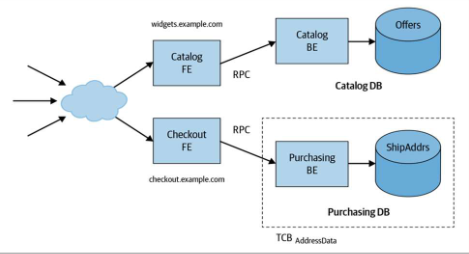
\includegraphics{images/tcb_decomposition.png}
   \caption{TCB Decomposition}
   \label{fig:tcb_decomposition}
\end{figure}


\section{Design for Change}

"\textit{Design for Change}" i.e. design to allow changes to disable new \textit{vulnerabilities}.
This poses many software engineering issues, but focusing only on security ones,
we can first consider which attributes should \textit{changes} {---}in a system{---} have:
\begin{enumerate}
   \item Incremental
   \item Documented
   \item Tested
   \item Isolated
   \item Qualified
   \item Staged i.e. check the benefit of the n-th change before applying the
   n+1-th change
\end{enumerate}

Note that Zero-day are not the only critical vulnerabilities;
important questions are:
\begin{itemize}
   \item "is this vulnerability currently exploited?"
   \item "is this vulnerability in the attack surface or can it be reached from the surface = an attack chain from the surface?"
\end{itemize}
Based on the answers to the previous questions, a \textbf{patching policy} chosen;
Generally patches are distributed using two distribution channels
\begin{enumerate}
   \item \textbf{low} risk vulnerabilities $\Rightarrow$ according to scheduling policy
   \item \textbf{high} risk vulnerability $\Rightarrow$ immediate patch to minimize the ris
\end{enumerate}

\section{Design for Resilience}

Each system layer should be designed to be \textbf{independently resilient}, implementing defense in depth among the
layers.

Compute the cost of prioritizing each feature, in order to understand which features are critical
enough to be sustained and which are less important and can be throttled or disabled.\\
\textbf{Compartmentalize} the system along clearly defined boundaries to promote the
independence of the isolated functional parts, achieving both \textit{segmentation} and \textit{isolation}.

Reduce \textit{reaction time} by \textbf{automating} as many of your resilience measures as possible, exploiting
intrusion detection, anomaly detection and pattern matching;
Also periodically validate resilience properties to ensure the effectiveness of the system.

\subsection{Risk assessment perspective}
Both attackers and defenders assess a target for weaknesses, but while \textit{attackers} perform \textbf{reconnaissance} against targets, find weaknesses, and model their
intruisons and the related attacks,
the \textit{defenders} instead (should) \textbf{know} the system, allowing for the assessment to be much more precise and comprehensive, 
but the defender has to implement \textit{remediations}, not attacks, which is very different.
The crucial point here is to understand that an \textit{attacker} is \textbf{\underline{not}} a \textit{defender}.
\begin{center}
   Defense is more effective if the defender understands the attacker methods and the more the defender understands the attacker methods\footnote{MITRE ATT\&CK matrix} the more the benefit is amplified.
   \nl

   \textit{"Enemy is the master"}
\end{center}

\subsection{Degradation}
The general idea is that if a system cannot resist to adversaries, then it can {--}and should{--} \textbf{limit} the blast radius of attacks.

The system layers are complementary, with each layer anticipating the weak
points or likely failures of the previous on;
designing for defense in depth assumes system components or even entire systems can fail due to physical damage, hardware malfunction, or an intrusion.

To control degradation, 
select properties to disable when specific circumstances
arise, while doing all you can to protect the system security.
By designing multiple response options for these events, the system can have controlled
\textbf{\textit{proactive} breakpoints} rather than a chaotic collapse;
in other words, we can "design" even \textit{crashes}.
\nl

For what concerns the "\textbf{blast radius}",
controlling it means \textit{compartmentalizing} the impact of an event, 
as, for instance, compartments on a ship grant resilience against the whole ship sinking;
security breach or traffic overload in one compartment should not jeopardize all compartments.
To this extent, when designing for resilience, there should be \textbf{compartmental barriers} that constrain both attackers and accidental failures, creating \textbf{failure domains} and 
allowing to better tailoring and automation of responses.

The principle behind compartmentalization is to isolate system elements and enable and control the
interactions essential for their intended purpose.
Compartmentalization can happen in two ways:
\begin{enumerate}
   \item Parallel decomposition
   \item Clustering
   \begin{enumerate}
      \item Containers
      \item VMs
      \item Phyisical machines
   \end{enumerate}
\end{enumerate}

\section{Trusted Platform Module}
\begin{figure}[htbp]
   \centering
   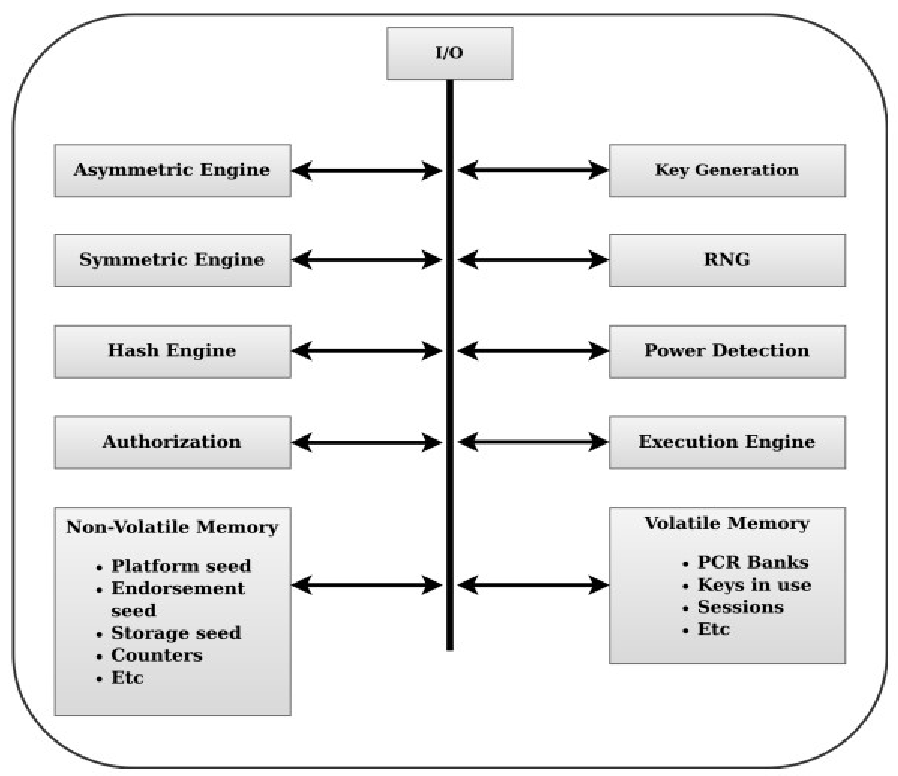
\includegraphics{images/tpm.png}
   \caption{TPM}
   \label{fig:tpm}
\end{figure}

Usually this protected chips are used to perform the \textbf{hash} of software running on nodes,
to ensure that the software has not been manipulated,
allowing a system to \textbf{trust} another one.
More generally , \textit{Remote Attestation Procedures} (\texttt{RAT}s) forsee one an \textit{Attester} peer which produces
believable information {--}\textit{Evidence}{--} about itself to enable a remote \textit{Challenger}\footnote{aka "Relying Party"} peer to decide whether the \textit{Attester} is a trustworthy peer
or not;
\texttt{RAT}S are facilitated by an additional vital party, the \textit{Verifier}.


\subsection{AWS Nitro System}
An EC2 server is made up of one or more \textbf{Nitro Cards} and a main system
board that contains the host CPUs and memory.

Nitro Cards are dedicated hardware components with 64-bit processing
capabilities and specialized \textit{Application Specific Integrated Circuits}
(\texttt{ASIC}s) that operate independently from the system; 
they implement all the outward-facing control interfaces used by the EC2 service to provision and manage computer, memory, and storage.

Three key components of the Nitro System, provide faster innovation, enhanced
security, and improved performance:
\begin{enumerate}
   \item \textit{Purpose-built Nitro Cards}\\
   Hardware devices designed by AWS that
   provide overall \textbf{system control} and input/output (\texttt{I/O}) virtualization
   independent of the main system board with its CPUs and memory.
   \item \textit{The Nitro Security Chip}\\
   Enables a \textit{secure boot} process based on a
   hardware \textbf{root of trust}, the ability to offer bare metal instances, as well as
   defense in depth to protect the server from unauthorized modification of
   system firmware.
   \item \textit{The Nitro Hypervisor}\\
   A minimized and firmware-like \textbf{hypervisor} to
   provide strong isolation, and performance nearly indistinguishable from a metal server.
   A limited and carefully designed component intentionally minimized and built with the capabilities to perform its required functions, and no more.\\
   The meticulous exclusion of non-essential features from the Nitro
   Hypervisor eliminates entire classes of bugs that other hypervisors
   can suffer from (remote networking attacks or driver-based privilege
   escalations).
   Besides, even in the unlikely event of a bug in the Nitro Hypervisor that allows
   access to privileged code, there is an \textbf{inhospitable environment} to any
   potential attacker due to the \textit{lack of} standard operating system
   features such as interactive shells, filesystems, common user space
   utilities, or access to resources that could facilitate lateral movement
   within the larger infrastructure
   \note{(harden your system \textit{S\&S})}

\end{enumerate}

In the Nitro System there is a \textbf{Nitro Controller} which provides the hardware \textbf{root of trust} for the overall system.
It is responsible for
managing all other components of the server system, including the firmware
loaded onto the other system components;
It is the exclusive gateway between the physical server and the control planes for EC2, EBS and VPC, 
and it operates together with Nitro Cards as a single domain.

A \textbf{Security chip} links the domain of the Controller to the domain of the external component that controls the system's main board (where the security chip usually resides).


By design there is \textbf{no operator} access, 
meaning there is no mechanism for systems or
persons to log in to EC2 Nitro hosts, access memory of EC2 instances
or any customer data stored on local encrypted instance storage or
remote encrypted EBS volumes.\\
If any AWS operator, even with the highest privileges, needs to do
maintenance work on an EC2 server, they can only use a limited set of
authenticated, authorized, logged, and audited \textit{administrative APIs}.
\textit{None} offers access customer data on the EC2 server.\\
Clearly this leads to not-so-easy debugging operations.

\section{Other resilience concepts}
\subsection{Graceful Degradation}
Essential and difficult choices should be carefully made in advance, not during an incident while being "under pressure".
Free up resources, thus decrease failed operations, by disabling infrequently used
features, least critical functions, or high-cost service capabilities,
prioritizing instead important features and functions.
Improving the system capacity to absorb load or failure supports all other
resilience mechanisms—and buys more time for response.

\begin{figure}[htbp]
   \centering
   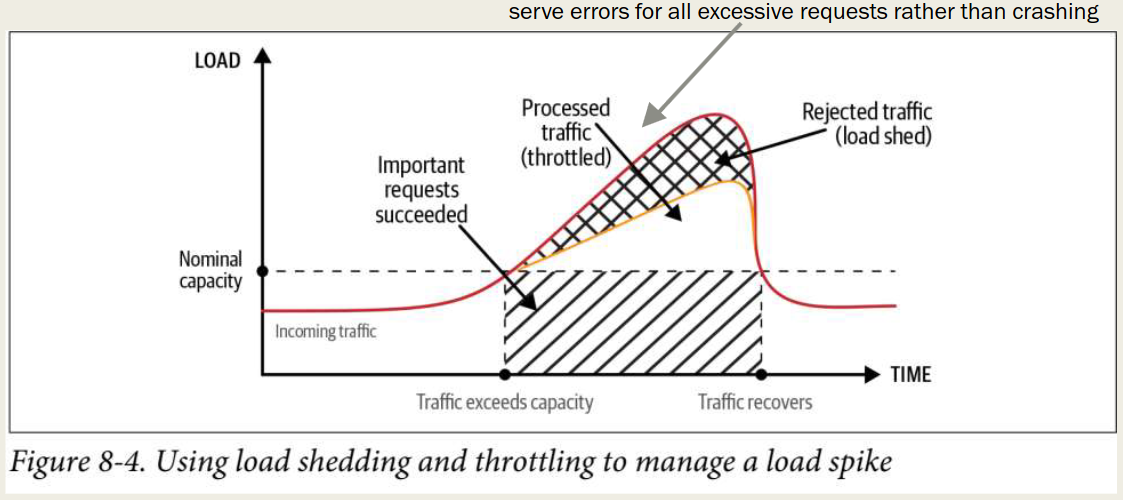
\includegraphics{images/graceful_degradation.png}
   \label{fig:graceful_degradation}
\end{figure}

\subsection{Failure Management}
\textbf{Failure management} should balance between optimizing for \underline{reliability} by failing
\textit{open} (safe) and optimizing for \underline{security} by failing \textit{closed} (secure).\\
To maximize \textbf{reliability}, a system should resist failures and serve as much as possible in face of uncertainty, even if integrity is not intact.\\
$\Longrightarrow$ If ACLs failed to load, the default ACL is \textit{"allow all"}

To maximize \textbf{security} instead, a system should lock down \textit{fully} in uncertainty.
If it cannot verify integrity the system can’t operate and should protect itself as much as possible.\\
$\Longrightarrow$ If ACLs failed to load, the assumed default ACL is \textit{"deny all"}
\begin{center}
   "Emergency exit doors" need \textit{fail safe} rather than \textit{fail secure} ones.
\end{center}

Security-critical operations should not \textit{fail open} because an attacker would be able to degrade system security through simple DoS attacks(think of a firewall),
but a controlled degradation of security-critical operations is possible.
A lower-cost component could replace failing security controls apllying stronger (possibly simpler) controls, making attacks to the default security controls \textit{not} effective, enhancing \textbf{resilience}.

TODO slide $[7...16]$ fatte velocemente
\nl

A strategy adopted by Google is to limit an attacker’s impact using the \textbf{location} hosting a service to prevent
an adversary who has compromised a datacenter to read data in other ones:
\textit{location-based} cryptographic compartments limit access to applications and
their stored data to specific locations, containing the \textit{blast radius} of attacks.



\subsection{Continous Validation}

\subsection{Observations}
All Google strategies are based on the fact that they have a huge number of resources all around the world.
They neglect hardware faults,
because they can easily fix by migrating software from a physical machine to another,
making hardware failures not so critical.

Amazon's approach instead is focuses also on physical aspects.

A feature of almost any cloud application is the adoption of multiple copies of resources, each managed by a distinct server and with a load balancer that can also change the number of copies.


